\section{Studying the presence of diabetes}

\frame{%
    \frametitle{Why diabetes?}

    \begin{itemize}
        \pause\item Of interest to the health board
        \pause\item Discussed widely in literature
        \pause\item Acts as an example for looking at condition-based slices
    \end{itemize}
}

\subsection{Distributions of key attributes and demographic information}

\frame{\frametitle{Number of spells associated with a patient}
    \centering
    \includegraphics[width=\imgwidth]{no_spells_hist/main.pdf}
}

\frame{\frametitle{Length of stay}
    \centering
    \includegraphics[width=\imgwidth]{los_hist/main.pdf}
}

\frame{\frametitle{Net cost of a spell}
    \centering
    \includegraphics[width=\imgwidth]{netcost_kde/main.pdf}
}

\frame{\frametitle{Number of diagnoses in an episode}
    \centering
    \includegraphics[width=\imgwidth]{no_diag_hist/main.pdf}
}

\frame{\frametitle{Number of procedures in an episode}
    \centering
    \includegraphics[width=\imgwidth]{no_proc_hist/main.pdf}
}

\frame{\frametitle{Distribution of age}
    \centering
    \includegraphics[width=\imgwidth]{age_hist/main.pdf}
}

\subsection{Correlation}

\frame{\frametitle{Pairwise correlation}
    \centering
    \includegraphics[width=\imgwidth]{corr_heatmap/main.pdf}
}

\subsection{Measuring variation and relative importance}

\frame{\frametitle{Cost variation}
    \centering
    \includegraphics[width=\imgwidth]{cost_variation/main.pdf}
}

\frame{\frametitle{Component contribution to net costs}
    \centering
    \includegraphics[width=\imgwidth]{cost_contribution/main.pdf}

}

\frame{\frametitle{Relative importance}
    \centering
    \includegraphics[width=\imgwidth]{cost_bubble_plot/main.pdf}
}

\frame{\frametitle{Components of interest (large contribution)}
    \centering
    \includegraphics[width=\imgwidth]{large_component_violinplots/main.pdf}
}

\frame{\frametitle{Components of interest (medium contribution)}
    \centering
    \includegraphics[width=\imgwidth]{middling_component_violinplots/main.pdf}
}

\subsection{Resource consumption}

\frame{\frametitle{Resource consumption}
    The definition of diabetic resource consumption will be based on three
    measures:

    \begin{itemize}
        \pause\item Proportion of total admissions
        \pause\item Average length of stay
        \pause\item Proportion of net cost spent
    \end{itemize}

    \pause%
    This method will has its flaws but allows for the analysis of how these
    measures evolve.
}

\frame{\frametitle{Proportion of admissions}
    \centering
    \includegraphics[width=\imgwidth]{admissions/main.pdf}
}

\frame{\frametitle{Average length of stay}
    \centering
    \includegraphics[width=\imgwidth]{los_time/main.pdf}
}

\frame{\frametitle{Proportion of net costs}
    \centering
    \includegraphics[width=\imgwidth]{netcost_proportions/main.pdf}
}

\subsection{Conclusions}

\frame{\frametitle{Conclusions}
    \begin{itemize}
        \item Resource consumption seems to be relatively consistent for
            patients presenting diabetes
        \item Cost components have smaller variations than \-- and are
            comparablein their contributions to \-- non-diabetic patients
    \end{itemize}
}
